\documentclass{article}
\usepackage[utf8]{inputenc}
\usepackage{amsmath}
\usepackage{graphicx}
\usepackage{float}
\usepackage[font=scriptsize,labelfont=bf]{caption}
\usepackage{hyperref}
\usepackage{subfig}

\title{COMP6247 : Recursive Least Square Assignment}
\author{Thanakorn Panyapiang\\
(31446612, tp2n19@soton.ac.uk)}
\date{}

\begin{document}
\maketitle

\section{Recursive Least Square Derivation}
I have studied the derivation of the Recursive least sqaure algorithm.

\section{Gradient Descent}

The solution estimated using the pseudo inverse, gradient descent, and stochastic gradient descent is shown in Fig \ref{fig:pi}, \ref{fig:gd}, and \ref{fig:sgd} respectively. The global trend of the learning curve in both gradient descent solutions is similar, as the squared error reduces over time and the decrease is significant at the first few iterations before stabilize later. However, it can be noticed clearly that while the curve is completely smooth, the learning curve fluctuates on the stochastic solution. This behavior is the result of adjusting the model using a single data point's gradient because its direction could be different from the total gradient.

\begin{figure}[H]
\begin{center}
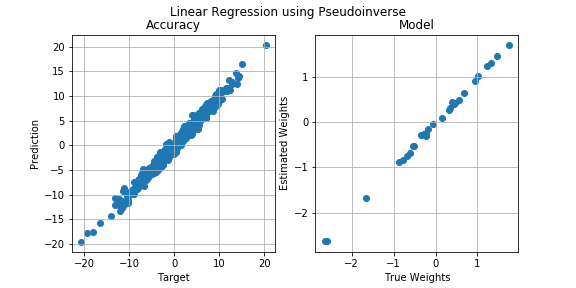
\includegraphics[scale=0.25]{PI.png}
\captionof{figure}{Pseudoinverse solution}
\label{fig:pi}
\end{center}
\end{figure}

\begin{figure}[H]
\begin{center}
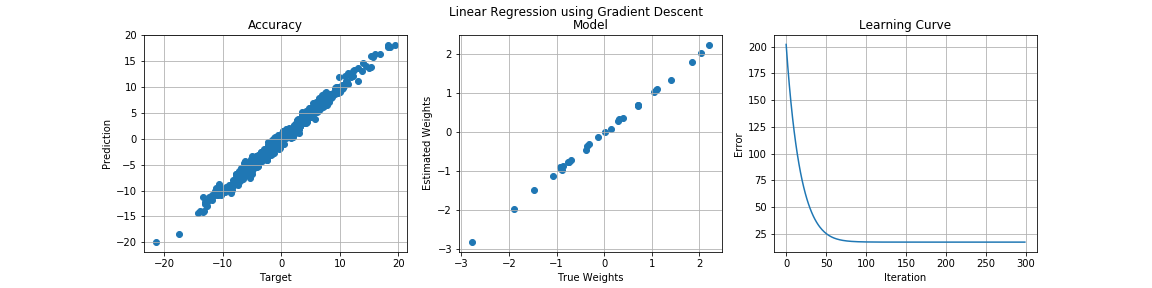
\includegraphics[scale=0.3]{GD.png}
\captionof{figure}{Gradient descent solution}
\label{fig:gd}
\end{center}
\end{figure}

\begin{figure}[H]
\begin{center}
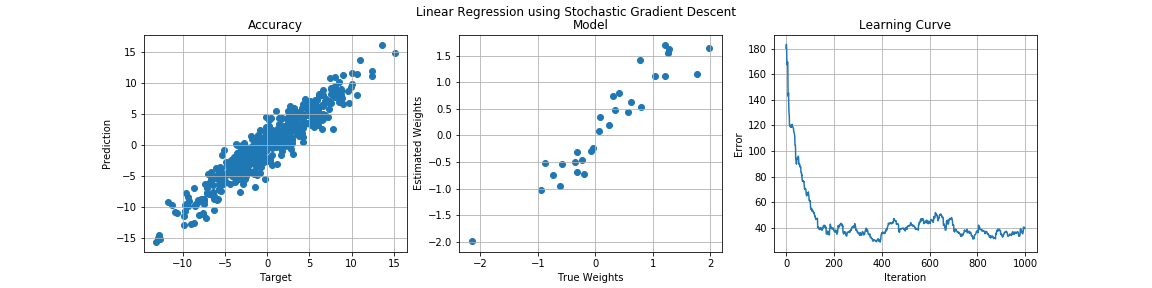
\includegraphics[scale=0.3]{SGD.png}
\captionof{figure}{Stochastic gradient descent solution}
\label{fig:sgd}
\end{center}
\end{figure}

There are several options for solving stochastic gradient descent issue. The easiest one would be to have a small learning rate so that each model adjustment is small as shown in Fig \ref{fig:sgd-improve}a, but it may decrease the speed of convergence.  

The more efficient approach for solving this problem is \textit{learning rate decay}. The principle of the technique is to reduce the learning rate over time. Learning rate decay allows the model to be updated quickly at the beginning so it can reach the global minimum. Once it is close to the global minimum, the model adjustment will be smaller to prevent overshoot. Fig \ref{fig:sgd-improve}b shows the learning curve of stochastic gradient descent with the same parameter as Fig \ref{fig:sgd} after applying the learning rate decay. It can be observed that the learning curve is still noisy at the beginning, but the model start to converge once the learning rate becomes low after around 200 iterations. 

\begin{figure}[H]
    \centering
    \subfloat[Small learning rate]{{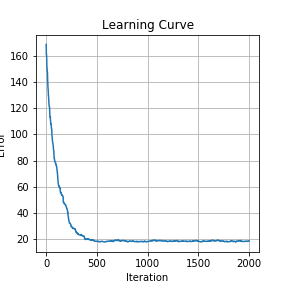
\includegraphics[scale=0.4]{SGD_small_lr.png} }}%
    \qquad
    \subfloat[Learning rate decay]{{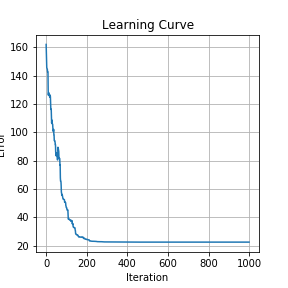
\includegraphics[scale=0.4]{decay-SGD.png} }}%
    \caption{Improving SGD convergence}%
    \label{fig:sgd-improve}%
\end{figure}

\section{Recursive Least Square}

The solution obtained from Recursive Least Square algorithm is show in Fig \ref{fig:rls}. The learning curve obsurved from the algorithm is very similar to stochastic gradient descent. In addition, as the dimention of data increase, the number of iteration which the algorithm uses before converge is higher. The result of this experiment is shown in Table \ref{tab:rls-dim}.
\begin{figure}[H]
\begin{center}
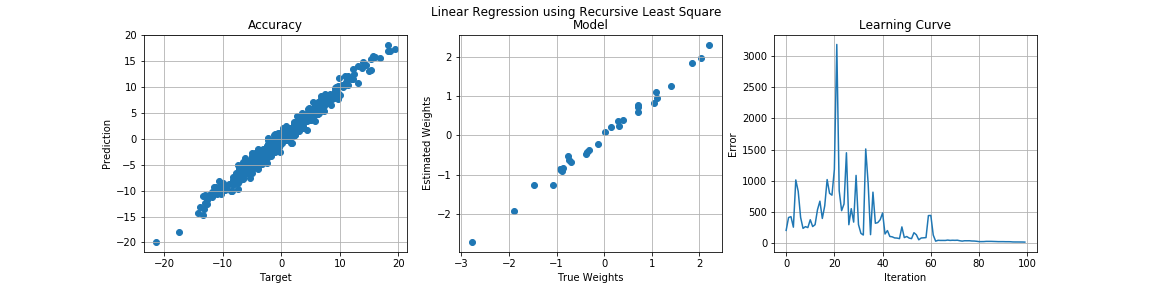
\includegraphics[scale=0.35]{RLS.png}
\captionof{figure}{Recursive least sqaure solution}
\label{fig:rls}
\end{center}
\end{figure}

\begin{table}[H]
\begin{tabular}{cccc}
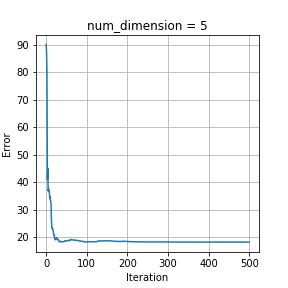
\includegraphics[scale=0.3]{RLS-5D.png} &
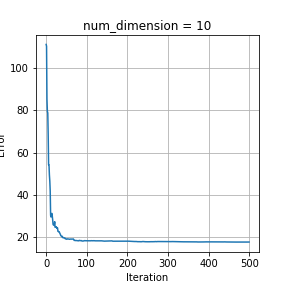
\includegraphics[scale=0.3]{RLS-10D.png} &
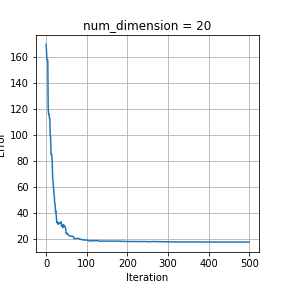
\includegraphics[scale=0.3]{RLS-20D.png} &
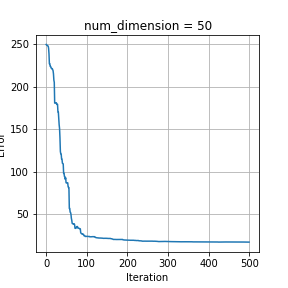
\includegraphics[scale=0.3]{RLS-50D.png}
\end{tabular}
\caption{Speed of convergence compare to number of dimensions}
\label{tab:rls-dim}
\end{table}

\section{Recursive Least Square on UCI dataset}
The data used in this section is the \textit{Auto MPG} dataset(\url{https://archive.ics.uci.edu/ml/datasets/auto+mpg}). With the same number of iterations, it turns out that \textit{Recursive least sqaure} algorithm performs slightly better in terms of total sqaured error. Regarding the speed of convergence, Recursive least square converges much faster at the beginning and become stable since around 400 iterations.

\begin{table}[H]
\begin{center}
\begin{tabular}{cc}
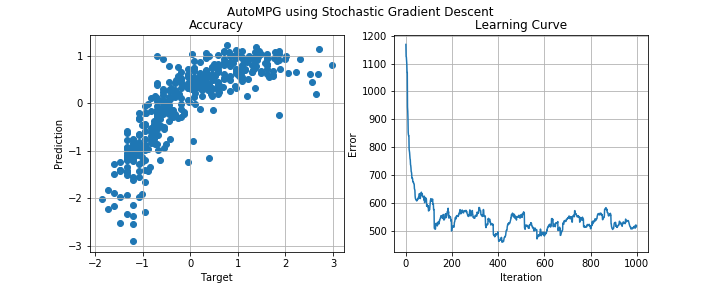
\includegraphics[scale=0.5]{MPG-SGD.png} &
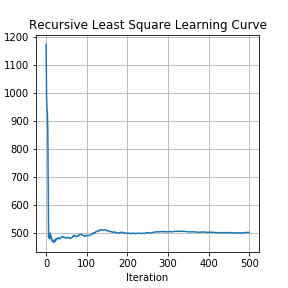
\includegraphics[scale=0.5]{MPG-RLS.png}
\end{tabular}
\end{center}
\end{table}

\end{document}
